\subsubsection{Central de Atendimento}
A Central de Atendimento/ Estação Base do VANT, será um local, qual será responsável por controlar toda a operação de atuação do VANT, desde o atendimento da chamada, ao desenvolvimento do plano de voô do mesmo. É responsabilidade do controlador auxiliar no uso do desfibrilador em casos de emergência. Sendo que, tal Base, estará sempre acompanhando o atendimento ao paciente e monitorando o funcionamento do VANT, através da alta gama de sensores e câmeras espalhadas pelo equipamento.

Não há qualquer requerimento especificado para o uso do software de controle, logo um computador padrão com capacidade média de processamento é o suficiente para o uso do software, se vê a importância de destacar que o computador deve possuir uma placa de rede para acesso à internet. Para o computador, foi escolhido um processador Intel I5 e 8GB de memória RAM, com essas configurações é garantido desempenho suficiente com um preço não elevado.  

O atendente que controlará o VANT e atenderá os chamados deve ser um médico socorrista com capacidade de auxiliar o uso do desfibrilador por pessoas leigas. Como a central funcionará 24 horas por dia, se vê necessário o uso de uma rotação de funcionários, levando em conta uma carga horária de 8 horas por dia para cada atendente. Por ser um serviço essencial que não pode ser interrompido, cada atendente deve possuir um substituto hábil de plantão.

Tal Central de Atendimento/Base Estação, apresentará as seguintes características:

\begin{itemize}
  \item 01 - Equipe, composta por 02 pessoas capazes de operar os equipamentos e softwares da Estação Base e do VANT
  \item 02 - Computadores DELL – InspironSmall Desktop \cite{DELL}
  \item 01 Gerador de Energia a Gasolina Portátil \cite{Gerador}
\end{itemize}


\subsubsection{Controlador Pixhawk}
O módulo Pixhawk piloto automático é um sistema muito eficiente em tempo real de operação. 
O software pode ser atualizado com um bootloader USB (gerenciador de boot USB), que é um programa simples com a 
função de acessar o disco do computador e carregar o sistema operacional na memória para assumir o controle do 
equipamento.

Os benefícios do sistema Pixhawk incluem \textit{multithreading}, ou seja, a capacidade de servir mais de um usuário ao 
mesmo tempo, um ambiente de programação Unix/Linux capaz de gerar novas funções de piloto automático, como 
escrita de missões e comportamento de voo. \cite{pix}
 
O módulo Pixhawk flagship pode ser utilizado visando as novas opções de periféricos, como sensor digital de velocidade do ar, o suporte para um indicador LED externo multicor e um magnetômetro externo. Todos os periféricos são automaticamente detectados e configurados. \cite{pix}

\subsubsubsection{Especificações}

\textbf{Processador}
\begin{itemize}
	\item 32-bit ARM Cortex M4 com FPU;
	\item 168 Mhz/256 KB RAM/2 MB Flash;
	\item 32-bit \textit{failsafe co-processor}.
\end{itemize}

\textbf{Sensores}
\begin{itemize}
\item MPU6000 com aceleração principal e giroscópio;
\item ST Micro 16-bit giroscópio;
\item ST Micro 14-bit acelerômetro /magnetmetro  MEAS barômetro.
\end{itemize}

\textbf{Alimentação}
\begin{itemize}
\item Controlador possui um diodo ideal com \textit{failover} automático;
\item Servo anteparo de alta potência (7V) e alta corrente de propensão;
\item Todas as saídas periféricas com \textit{over-current}, assim como todas as entradas ESC, possuem proteção.
\end{itemize}

\textbf{Interfaces}
\begin{itemize}
\item 5x UART com porta serial, 1 componente \textit{high-power}, 2x HW com controle de fluxo;
\item \textit{Spektrum} DSM/DSM2/DSM-X entrada de satélite;
\item \textit{Futaba} S.BUS entrada ( saída não implementada);
\item PPM sinal de soma;
\item RSSI (PWM ou tensão) entrada;
\item I2C, SPI, 2x CAN, USB;
\item 3.3 e 6.6 ADC entradas.
\end{itemize}

\textbf{Dimensões}
\begin{itemize}
\item Peso 38 g (1.3 oz);
\item Largura 50 mm (2.0”);
\item Altura 15.5 mm (.6”);
\item Comprimentob 81.5 mm (3.2”).
\end{itemize}
\begin{figure}[H]
	\centering
	  \includegraphics[keepaspectratio=true,scale=0.6]{figuras/pix1.eps}
	\caption{Visão geral da Pixhawk. Fonte \cite{pixhawk}}
	\label{fig:pix1}
\end{figure}

\begin{figure}[H]
	\centering
	  \includegraphics[keepaspectratio=true,scale=0.5]{figuras/pix2.eps}
	\caption{Entradas  de comunicação de dados  do Pixhawk. Fonte \cite{pixhawk}}
	\label{fig:pix2}
\end{figure}

\pagebreak
\begin{figure}[H]
	\centering
	  \includegraphics[keepaspectratio=true,scale=0.6]{figuras/pix3.eps}
	\caption{Plano de alimentação da PixHawk. Fonte \cite{pixhawk}}
	\label{fig:pix3}
\end{figure}

\begin{figure}[H]
	\centering
	  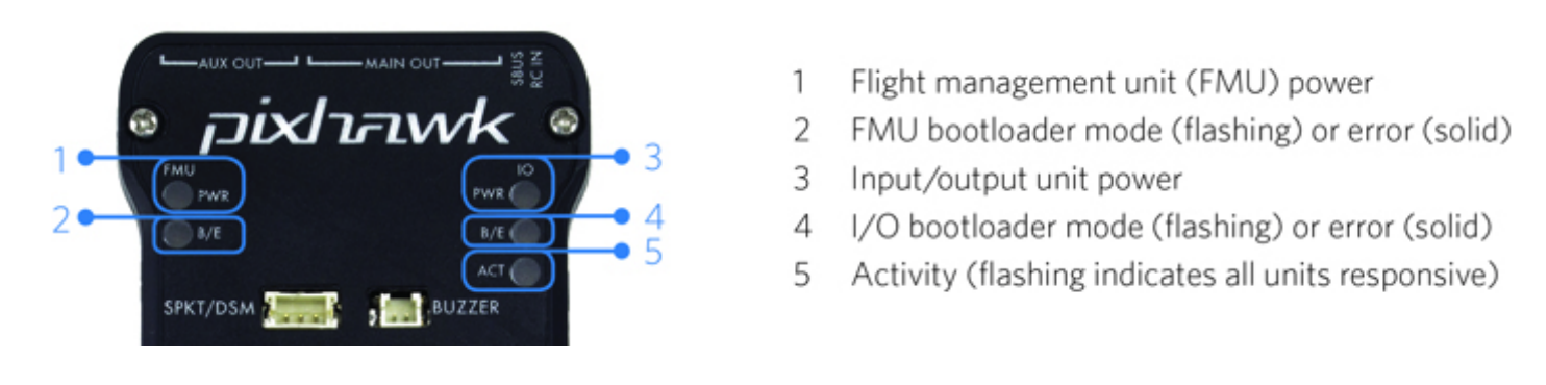
\includegraphics[keepaspectratio=true,scale=0.6]{figuras/pix4.eps}
	\caption{Conexões da superfície da PixHawk. Fonte \cite{pixhawk}}
	\label{fig:pix4}
\end{figure}

\begin{figure}[H]
	\centering
	  \includegraphics[keepaspectratio=true,scale=0.6]{figuras/pix5.eps}
	\caption{Diagrama dos conectores da PixHawk. Fonte \cite{pixhawk}}
	\label{fig:pix5}
\end{figure}

\begin{figure}[H]
	\centering
	  \includegraphics[keepaspectratio=true,scale=0.6]{figuras/pix6.eps}
	\caption{Atribuições de pinos do conector da PixHawk. Fonte \cite{pixhawk}}
	\label{fig:pix6}
\end{figure}

\subsubsection{Correntes de saída da placa controladora}

	Considerando os seguintes componentes ligados a placa:

	\begin{itemize}

		\item 01 \textit{ESC Red Brick 200A Brushless;}
		
		\item 08 \textit{Motores TAROT 4114 Higj Power Brushless; }
		
		\item 01 \textit{RadioTelemetry (3DR RADIO V2);}
		
		\item 01 \textit{PPM Sum Receiver;}
		
		\item 01 \textit{GPS and Compass kit 3DR; }
		
		\item 01 \textit{Buzzer;}

	\end{itemize}

	De acordo com o \textit{datasheet} de cada componente podemos estimar a corrente total de saída da placa controladora. 
	Assim, sabendo que cada motor será capaz de carregar 2.15 (Kg), e determinado que chegará uma tensão de 22.2 (V) no motor, 
	devido a bateria utilizada, o mesmo necessitará de uma corrente de 14.5 (A). \cite{helipal}.
	Sabendo que o ESC utilizado será capaz de controlar e suportar os oito motores, a sua corrente deverá de ser oito vezes a 
	corrente do motor, pois a corrente deve chegar no ESC e se dividir para os oito motores, seguindo a seguinte expressão: 

	\begin{center}
 
	$I_{esc} = 8*I_{motor}$
	$I_{esc}$ = 116 (A)
	
	\end{center}

	Ao analisar o \textit{datasheet} de tal componente, sabe-se que o mesmo é capaz de suportar uma corrente de até 200 (A), 
	sendo a corrente calculada dentro do limite estabelecido.\footnotemark
	Para o próximo componente, 3DR RADIO V2, foram obtidas as seguintes informações: 
	
	\footnotetext{http://www.shuziguangxi.com/pt/Red-Brick-200A-ESC-Brushless-ESC-OPTO-NO-BEC-200A\%28OPTO\%29-p-77974.html}
	\indent Recebe uma corrente de 25 (mA); \cite{radio}.\\
	\indent Transmite uma corrente de 100 (mA); \cite{radio}. 
	
	No caso, como estamos interessados nos componentes ligados a placa consideramos apenas a corrente que o rádio recebe, sendo essa de 25 (mA).
	Tomando como referência o \textit{datasheet} do PPM Encoder da 3DR não foi encontrado nenhum valor de corrente referente ao funcionamento do mesmo. Assim, considera uma corrente muito pequena, não influenciando nos seguintes cálculos. \cite{enconder}.
	Para o módulo \textit{GPS and COMPASS}, temos uma série de componentes em seu interior que consomem uma corrente especifica, sendo eles e suas correntes, respectivamente: 

	 \begin{itemize}
		\item \textit{LEA-6 Series: 22 ($\mu$A)}\cite{product};
		
		\item \textit{NEA-7: 10 ($\mu$A)} \cite{datasheet};
		
		\item \textit{Taoglas Antena: -- (não encontrada)} \cite{antena2};
		
		\item \textit{Maxim Amplifier: 4.1 ($\mu$A)}\cite{maximin};
	\end{itemize}		
	Obtendo assim uma corrente final de 14.122 (mA).

Por fim, temos a corrente do Buzzer, que ao analisar o seu \textit{datasheet}, encontramos que sua corrente máxima é de 30 (mA). \cite{felcodis}.
	Assim, podemos estimar uma corrente total de saída da Placa Controladora somando todas as correntes dos componentes ligados a ela, sendo que deve levar em conta que o ESC estará ligado em série com os motores, considerando apenas a corrente do ESC para a soma, assim sendo: 

	\begin{center}

		$I_{total}$ = $I_{esc}$ + $I_{tl}$ + $I_{ppm}$ + $I_{gpsc}$ + $I_{bzz}$

		$I_{total}$ =$116 (A)$ + $25 (mA)$ + 0 + $14.122 (mA)$ + $30 (mA)$

		$I_{total}$ = $116.07 (A)$

	\end{center}
	
\indent $I_{esc}$: Corrente do ESC;

\indent $I_{tl}$: Corrente do \textit{RadioTelemetry} (3DR RADIO V2);

\indent $I_{ppm}$: Corrente do PPM \textit{Sum Receiver};

\indent $I_{gpsc}$: Corrente do \textit{GPS and Compass} kit 3DR;

\indent $I_{bzz}$: Corrente do \textit{Buzzer}; 

	

\subsubsection{Funcionamento do VANT}

Os VANT's por serem um tipo de veículo de pequeno porte e em conseqüência a miniaturização de seus componentes eletrônicos e seu barateamento, têm-se sua utilização gradativamente aumentada nas mais diversas áreas, como: vigilância, análise ambiental, missões militares e busca e salvamento de pessoas tanto em auto mar, como em áreas de pouco acesso. \cite{Branco}

O VANT projetado,será composto por um complexo sistema integrado, apresentando cinco sub-módulos principais  que trabalham em conjunto afim de obter uma alta plataforma de observação e atuação.

Sendo esses módulos, baseados em \citeonline{pastor}.

\begin{itemize}
	\item Estrutura do VANT – Uma estrutura simples, leve, aerodinamicamente eficiente e com uma plataforma estável, capaz de oferecer uma otimizização na qualidade de voo do mesmo. 
	\item Controlador do VANT – Para realizar todo o processo de controle, comunicação externa e autonomia de voo do VANT, será utilizado o controlador PIXHAWK, da empresa 3D Robotcs, um sistema de computador concebido para coletar informações aerodinâmicas através de um conjunto de sensores(acelerômetros, giroscópios, magnetômetros, sensores de pressão, GPS, etc.), de modo a pilotar automaticamente o VANT.
	\item Caixa de Sensoriamento - Um conjunto de sensores compostos por câmeras de TV, sensores infravermelho, sensores térmicos, etc., para reunir informações que podem ser parcialmente processadas \textit{on-board}, pelo próprio controlador do VANT, ou transmitidas a uma base estação, para posterior análise.
	\item Estação Base – Uma equipe de chão, situada em uma região próxima a área de atuação do VANT, destinada a monitorar o desenvolvimento do voo, acompanhar e orientar o atendimento de emergência e eventualmente operar o VANT, caso ocorra alguma falha técnica. 
	\item Infraestrutura de Comunicação - Uma mistura de mecanismos, equipamentos e técnicas de comunicação (moldens de rádio,satcomm, links de microondas, etc.) que devem garantir um elo contínuo e estável entre o VANT e a estação de base. 
\end{itemize}


\begin{figure}[H]
	\centering
	  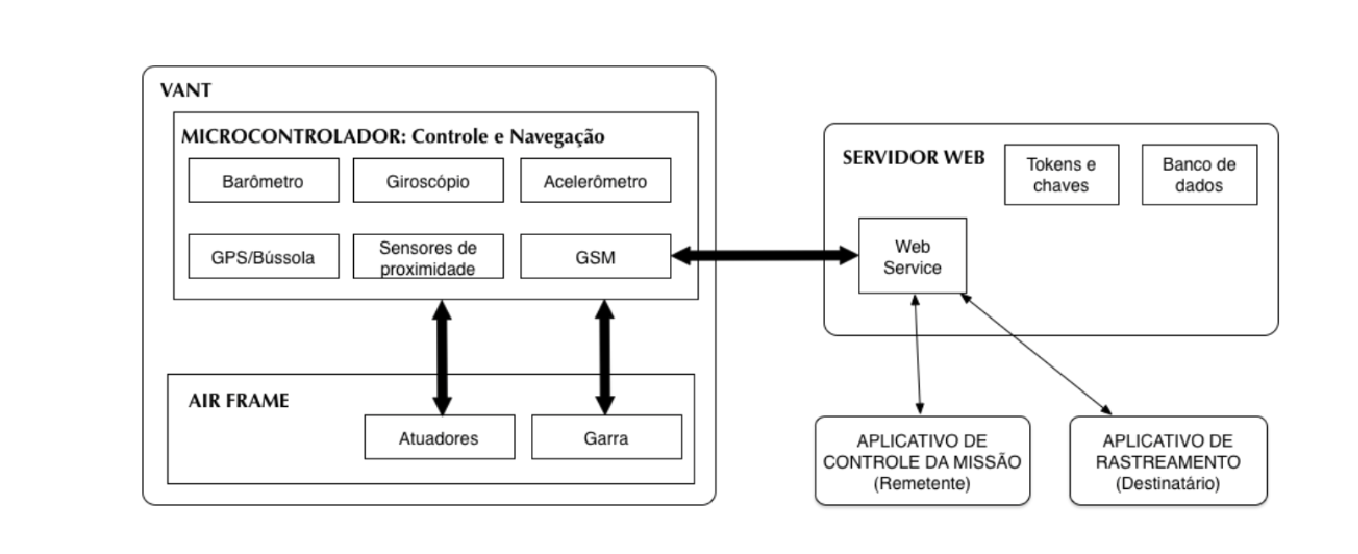
\includegraphics[keepaspectratio=true,scale=0.7]{figuras/diagrama.eps}
	\caption[Diagrama simplificado da comunicação do VANT com a Central.]{Diagrama simplificado da comunicação do VANT com a Central. Fonte \cite{Branco}}
	\label{fig:diagrama}
\end{figure}

A arquitetura de implementação do VANT utilizará microcontroladores, assim como sensores e módulos de transmissão de dados (Figura \ref{fig:diagrama}).
Os dados transmitidos entre o servidor na central de monitoramento, o VANT e os aplicativos (controle da missão e rastreador) 
seguirão um determinado padrão. Em caso de perda sinal, com a central de controle, o VANT será programado para que retorne 
automaticamente para a base de controle.

A Figura \ref{fig:esquemageral} mostra o esquema simplificado de montagem dos componetes do VANT.

\begin{figure}[H]
	\centering
	  \includegraphics[keepaspectratio=true,scale=0.6]{figuras/esquemageral.eps}
	\caption{Esquema de montagem do VANT. Fonte:\cite{esquematico}}
	\label{fig:esquemageral}
\end{figure}

\pagebreak



\subsubsection{Sistema de comunicação via rádio frequência}

Os sistemas de comunicação sem fio são baseados em campos eletromagnéticos
, e são ondas que transportam energia de um ponto ao outro, 
isso possibilita que haja comunicação sem a necessidade de uma conexão física dos fios \cite{VALLE1}. 

Para que haja a propagação do sinal de radiofrequência (RF) é necessário que o sinal seja conduzido por um cabeamento condutor até uma
antena que posteriormente irá irradiar através do ar os pulsos eletromagnéticos do sinal \cite{VALLE1}. 

A antena é um componente responsável por converter um sinal, do meio cabeado, em um sinal \textit{wireless} (sem fio) e vice-versa, 
como é possível
ver na figura \ref{fig:antena}. Os sinais irradiados no ar livre, em forma de ondas eletromagnéticas, propagam-se em linha reta e em 
todas as direções 
\cite{Rappaport2}. Com isso pode-se transmitir qualquer tipo de informação a um receptor remoto apenas utilizando a propagação dessas ondas 
eletromagnéticas.

\begin{figure}[H]
	\centering
	  \includegraphics[keepaspectratio=true,scale=0.6]{figuras/antena.eps}
	\caption{Transmissão radioelétrica de informação. Fonte: \cite{antena}}
	\label{fig:antena}
\end{figure}

\subsubsection{Radiofrequências}

O espectro eletromagnético da radiofrequência ocupa as frequências entre os 3 kHz e os 300 GHz. 

A figura \ref{fig:tabelafre} mostra as bandas de radiofrequência, o nome das respectivas e suas aplicações tradicionais.

\begin{figure}[H]
	\centering
	  \includegraphics[keepaspectratio=true,scale=0.6]{figuras/tabela.eps}
	\caption{Bandas de Radiofrequência. Fonte: \cite{tabela}}
	\label{fig:tabelafre}
\end{figure}

As ondas de radiofrequência de médias e baixas frequência (MB e ELF) possuem grandes comprimentos de onda, essa característica favorece a 
difração na atmosfera e garante que os obstáculos de grandes dimensões sejam contornados mais facilmente \cite{Rappaport2}.

Quanto maior a frequência menos é a capacidade de transmitir para distâncias muito longas ao nível da superfície terrestre \cite{VALLE1}. 

\begin{itemize}
	\item As ondas MF são as ondas utilizadas nas estações nacionais, permitindo difundir o som com maior qualidade, embora com menor alcance;
	\item As ondas LF são utilizadas nas estações de rádio que transmitem a nível mundial;
	\item As ondas ELF, que têm frequências extra baixas, são utilizadas quando tem-se grande obstáculos e necessita enviar uma informação. 
	\item As ondas HF e VHF, possuem pequenos comprimentos de ondas, geralmente sofrendo múltiplas reflexões na ionosfera e na superfície terrestre, não conseguem acompanhar a curvatura da Terra. São utilizadas em comunicações que não exigem grande alcance, mas quando é exigida a alta qualidade de som e imagem.
	\item As ondas UHF, SHF e EHF são utilizadas para comunicação com satélites, pois o seu comprimento de onda é muito pequeno e ele não sofre quase que refração nenhuma na atmosfera. 
\end{itemize} 

\subsubsection{Agência Nacional de Telecomunicações - ANATEL}

Para que seja criado um novo \textit{link} utilizando radiofrequência é necessário consultar a ANATEL, pois ela é responsável por 
manter o controle de todas as frequências utilizadas nas telecomunicações, para garantir que não exista interferências nas transmissões.

\begin{figure}[H]
	\centering
	  \includegraphics[keepaspectratio=true,scale=0.6]{figuras/anatel.eps}
	\caption{Atribuição de faixas de frequências na ANATEL. Fonte: \cite{anatel}}
	\label{fig:tabela}
\end{figure}


Para poder ter acesso a um canal de frequência é necessário cumprir o regulamento de uso do espectro de radiofrequências. 
Resolução Nº 259 de 19 de abril de 2001 (em anexo).

\subsubsection{Especificação do projeto da comunicação do VANT}

Para a comunicação será utilizado dois canais.

\begin{itemize}
	\item Um canal será responsável apenas pela comunicação dos dados referentes ao deslocamento, ele será para o controle do VANT, então será transmitido informações da trajetória que será seguida para o piloto automático e em caso de emergência o controle manual.
	\item O outro canal será para transmissão dos dados de vídeo e áudio.
\end{itemize}

\subsubsection{A comunicação e transmissão de dados }

O piloto automático guiará o VANT até a emergência. A central receberá a solicitação do veículo e com as orientações do local do 
socorro, ela irá mapear o percurso a ser seguido para chegar até o destino e enviará as informações.  
Essas informações referentes ao trajeto e coordenadas de 
GPS serão passadas de forma \textit{wireless} serialmente para o sistema e controladores do VANT. Para que isso aconteça, eles estarão conectadas 
por um canal de comunicação de radiofrequência, no caso já existente do corpo de bombeiros.

A central necessitará passar informações ao usuário referentes ao atendimento, também precisará ver o estado do paciente e ver se os 
procedimentos foram realizados conforme as instruções e as informações dos sinais vitais da vítima para entender a real situação dele. 
Com isso a central receberá um sinal de áudio e vídeo e o VANT receberá apenas o sinal de áudio da central, por onde o operador poderá
fazer as orientações necessárias.

\subsubsection{Projeto da comunicação do VANT}
A comunicação da central de atendimento e o VANT será através de um \textit{link} de radiofrequência, será criado um canal na faixa das VLF
\textit{(Very Low Frequency)}.

\begin{itemize}
	\item  A escolha dessa faixa de operação VHF foi devido à grande taxa de transferência;
	\item Qualidade das informações a serem transmitidas;
	\item Não se propaga por longas distâncias;
	\item A faixa das VHF são de 30MHz a 300 MHz;
	\item  O Canal de comunicação do VANT será nessa faixa de 39,020MHz que é a faixa utilizada pelo CBMDF.
\end{itemize}

\subsubsubsection{Áudio e Vídeo}

A qualidade de vídeo de 720p assume formato widescreen 16:9 e uma resolução vertical de 1280 pixels de um total de 0,92 milhão de pixels. 
A taxa de quadros utilizada será de 60fps (\textit{frames} por segundo). 

A câmera possibilitará a captura de vídeos e de áudio, para que seja transmitida pelo canal de rádio frequência. O vídeo será transmitido em 
720p e será utilizando o padrão de compressão de vídeo H.264.

\begin{center}
 $720p a 60 fps$
  Resolução
  $1280 x 720$
  Taxas de bits do vídeo
  Máxima: 6000 Kbps
\end{center}

Para o áudio, será utilizado áudio Estéreo será necessário uma faixa de 384 Kbps
Com isso o pacote a ser transmitido deverá ter taxa de transmissão mínima de cerca de 6384 Kbps. \footnotemark

\footnotetext{https://support.google.com/youtube/answer/1722171?hl=pt-BR}


\subsubsubsection{Taxa de transferência do canal}
Em 1928, Harry Nyquist, desenvolveu um estudo para a definição máxima de um canal de banda passante limitada e imune a ruídos, 
com isso ele chegou em  uma equação matemática que pode ser escrita da seguinte forma \cite{semente}:

\begin{equation}
 C = 2*W*Mm bps
\end{equation}

\indent C = capacidade do canal na ausência de ruído;

\indent W = frequência do sinal (largura de banda);

\indent Mm = a modulação multinível (2 bits, 4 bits, 8 bits, 16 bits...);

Considerando a melhor das hipóteses, considerando que esteja sendo utilizando uma codificação A/D de 16 bits, 
tem-se que a melhor transferência de bits é dado por: 

\begin{equation}
 39,020 MHz-33,48MHz=5,54MHz
\end{equation}

\begin{center}
 $C = 2*5,54* {10} ^ {6} *16=177280000=177,28 Mb/s$
\end{center}

Com essa taxa de transferência é possível existir a comunicação em vídeo e áudio entre o VANT e a central. 

\subsubsection{Análise de Custos}

\indent \textbf{Central}

\begin{itemize}
 \item Computador \textit{Dell Inspiron Small Desktop} com processador Intel I5, Windows 8.1 e monitor: R\$ 2659,00  \footnotemark
\footnotetext{\url{http://www.dell.com/br/p/inspiron-3647-small-desktop/pd?oc=cai3647w8s161315brp118w1&model_id=inspiron-3647-small-desktop}}

  \item Roteador D-Link DIR-615: R\$ 74,00

  \item Mouse óptico básico: R\$ 9,90 (não há mouse incluso com o computador) \footnotemark
    \subitem *Justificativa para escolha do mouse se precisar: Supre os requisitos e foi o mais barato encontrado
  \footnotetext{\url{http://www.kabum.com.br/produto/18614/mouse-multilaser-optico-usb-preto-mo130}}

  \item Internet GvT 15 mega: R\$ 69,90. \footnotemark
    \subitem *Mais barato que o equivalente da NET.
    \footnotetext{\url{http://www.gvt.com.br/PortalGVT/Residencial/Banda-Larga/Planos}}

  \item Média Salarial de socorristas: R\$ 1099,54 \footnotemark
    \footnotetext{\url{http://www.catho.com.br/profissoes/socorrista/o-que-faz-um-socorrista}}

  \item Cadeira de Escritório Office One Cinza – Seatwell: R\$ 125,00 \footnotemark
  \footnotetext{\url{http://www.walmart.com.br/produto/Moveis-e-Decoracao/Cadeiras-de-Escritorio/Seatwell/383807-Cadeira-de-Escritorio-Office-One-Cinza---Seatwell}}

  \item Mesa para Computador ME-4107 Branco – Tecnomobili: R\$ 199,00 \footnotemark
    \footnotetext{\url{http://www.walmart.com.br/produto/Moveis-e-Decoracao/Escrivaninhas/Tecnomobili/452689-MESA-DE-COMPUTADOR-BRANCO}}

  \item Headset Dazz 621102 Ajustável Preto: R\$ 24,90 \footnotemark
    \subitem(Para comunicação da central com os demais pontos necessários)
  \footnotetext{\url{http://www.walmart.com.br/produto/Acessorios-de-Tecnologia/Fones-de-Ouvido-e-Headsets/Dazz/423677-HEADSET-BLACK}}

  \item Custo total da central (2 computadores com mouse + roteador + 2 cadeiras + 2 mesas + 2 Headsets): R\$ 6109,60
  \item Custo mensal de manutenção de serviços (internet + 6 funcionários): R\$ 6667,14 



\end{itemize}


\indent \textbf{Controlador}

\begin{itemize}
  \item Valor do controlador, convertido para reais em 17 de junho de 2015: R\$ 611,97 
\end{itemize}
